\chapter{Bruits et parasites}
\section{Introduction}
Introduisons ce que sont bruits et parasites:
\begin{description}
	\item[Bruit] au sens strict (encore appelé "bruit de fond") est un signal à variation aléatoire d'origine \emph{interne} au dispositif étudié. Il est possible de le définir, de prévoir son niveau plancher à l'aide du dimensionnement
	\item[Parasites] signaux perturbateurs d'origine \emph{externe} au dispositif
\end{description}
Ces 2 phénomènes se présentent sous forme de signal analogique venant s'additionner au signal utile, entraînant ainsi sa dégradation. Une fois le signal utile perturbé, pas de marche arrière, d'où l'importance des ces concepts lors du dimensionnement.
\begin{table}[H]
	\centering
	\begin{tabular}{lcr}
		& \textbf{bruit} & \textbf{parasite} \\ \hline
		origine & interne & externe \\
		distribution & aléatoire & variable \\
		bande passante & "$\infty$" & limitée \\
		amplitude & faible & variable \\
		& "plancher" & arbitrairement bas \\
		modélisation & "facile" & difficile \\
		contre-mesures & conception & conception/remédiation \\ \hline
 	\end{tabular}
	\caption{Critères de distinction}
\end{table}
On remarque que:
\begin{itemize}
	\item contrairement au bruit qui possède généralement une amplitude plancher, calculable théoriquement, il est théoriquement impossible de réduire les parasites à un niveau arbitrairement bas.
	\item La modélisation des effets du bruit dans un système est ,dans le principe, simple. Au contraire, la modélisation des parasites est nettement plus difficile car ceux-ci sont constitués de plusieurs signaux plus déterministes dont il faut connaître les couplages avec le système étudié.
\end{itemize}
L'introduction des ces phénomènes relève tout l'intérêt des signaux numérique (au lieu d'analogique). En effet, alors qu'un signal analogique dégradé ne peut être restauré, il est possible généralement de restauré un signal numérique dégradé.\\
Un signal numérique n'est rien d'autre qu'un signal analogique dont certains niveaux représentent des valeurs discrètes portant une information (paliers, ex. 0=vrai, 1=faux) et dont chaque niveau peut varier dans certaines limite $\rightarrow$ marges de bruit.\\

Ainsi, si l'impact des bruits et parasites est inférieur à cette marge de bruit définie par la conception, il est possible de restaurer le signal numérique utile. Les signaux numériques présentent donc une meilleure robustesse face aux perturbations. Il sera néanmoins toujours nécessaire de limiter les perturbations (car marges de bruit limitées).
\section{Le bruit de fond}
\subsection{Introduction}
Le bruit de fond possède plusieurs caractéristiques:
\begin{itemize}
	\item fluctuation aléatoire fondamentale due à la nature elle-même du dispositif
	\item limite ultime de la résolution du dispositif (contrairement aux parasites)
	\item fondamentalement inévitable (jamais nul) mais sont influence sur la chaîne peut être minimisé
	\item origine générale en électronique: fluctuations de la densité des porteurs de charges (porteurs de charges = $e^-$ et trous, fonction de la température)
	\item observable sur une tension et/ou un courant
\end{itemize}
Il existe plusieurs type de bruit, comme le bruit de type gaussien (c-à-d qui suit une loi normale de moyenne et variance données $N(\mu,\sigma)$, \autoref{fig:densiteprobagauss})

\begin{figure}[H] 
	\centering 
\pgfmathdeclarefunction{gauss}{2}{%
	\pgfmathparse{1/(#2*sqrt(2*pi))*exp(-((x-#1)^2)/(2*#2^2))}%
}
	\begin{tikzpicture}[
	every pin edge/.style={<-},
	every pin/.style={fill=yellow!50,rectangle,rounded corners=3pt,font=\small}]
	\begin{axis}[every axis plot post/.append style={
		mark=none,domain=-3:3,samples=30,smooth},
	clip=false,
	axis y line=none,
	axis x line*=bottom,
	ymin=0,
	xtick=\empty,
	]
	\addplot {gauss(0,0.5)};
	\addplot {gauss(0,1)};
	\draw[dashed]  (axis description cs:0.5,0) node[below] {$\mu$} -- (axis description cs:0.5,0.92) ;
	\end{axis}
	\end{tikzpicture}
\caption{Bruit de type gaussien: densité de probabilité}
\label{fig:densiteprobagauss}
\end{figure}
On peut alors se demander qu'elle est la valeur maximale du bruit ? Prenons par exemple un bruit de valeur efficace $\SI{1}{\volt}$ (\autoref{fig:tensionbruitmax}). Il est tout à fait possible qu'au bout de $\SI{100}{\second}$ on ait un bruit 10 fois plus grand. C'est aléatoire, mais sa puissance rms est constante.
\begin{figure}[H] 
	\centering 
	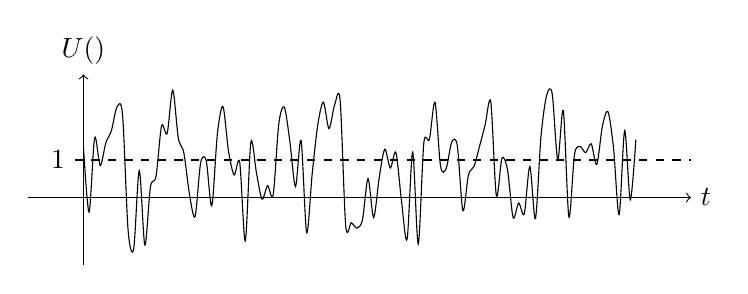
\begin{tikzpicture}[samples=100, domain=0:5*360]
	\begin{axis}[
	width=10cm, height=4cm,
	enlarge x limits=true,
	xtick=\empty,
	ytick=\empty,
	axis line style={->},
	axis lines*=middle,
	xlabel=$t$,
	ylabel=$U(\si{\volt})$,
	every axis x label/.style={
		at={(ticklabel* cs:1)},
		anchor=west,
	},
	every axis y label/.style={
		at={(ticklabel* cs:1)},
		anchor=south,
	},]
	\addplot [no markers, smooth] {sin(x)*sin(x)+rand};
	\draw[dashed] (axis description cs:0.07,0.55) node[left] {\SI{1}{\volt}} -- (axis description cs:1,0.55) ;
		\end{axis}
	\end{tikzpicture}
	\caption{Bruit de type gaussien: tension} 
	\label{fig:tensionbruitmax}
\end{figure}

\paragraph{Remarque:} la "valeur efficace" est une puissance mesurée, ce n'est pas le max
\subsection{Caractérisation mathématique}
\subsubsection{Définition de base}
Mathématiquement, le bruit est caractérisée par un \emph{signal temporel} (f.e.m) $E_b(t)$ avec les propriétés suivantes:
\begin{itemize}
	\item {\makebox[8cm]{fluctuation aléatoire $\Rightarrow$ moyenne nulle\hfill} $\overline{E_b(t)}=0$}
	\item {\makebox[8cm]{valeur quadratique moyenne non nulle\hfill} $\overline{E_b^2(t)} \neq 0$}
	\item {\makebox[8cm]{valeur efficace ("rms" = root mean square)\hfill} $E_b=\sqrt{\overline{E_b^2(t)}}$}
	\item {\makebox[8cm]{rapport signal/bruit SNR [dB]\hfill} $SNR=10\log\frac{\overline{E^2_s(t)}}{E_b^2(t)}$}
\end{itemize}
\subsubsection{Variation en fréquence}
À ces propriétés s'ajoutent:\begin{itemize}
	\item La valeur efficace dépend de la fréquence $\Rightarrow$ \emph{densité spectrale} de bruit $e_b^2(f)=\left.\frac{d\overline{E_b^2}}{df}\right|_f\quad [\si[per-mode=symbol]{\volt\squared\per\hertz}]$
	\item La couleur du bruit:
	\begin{itemize}
		\item bruit blanc: densité spectrale constante en fréquence (uniformément réparti en fréquence, \autoref{fig:bruitblanc})
		\item bruit rose: densité spectrale plus forte pour les basses fréquences (descente linéaire, \autoref{fig:bruitrose})
	\end{itemize}
\end{itemize}
\begin{figure}[H]
	\centering
	\subfigure[Bruit blanc]{\label{fig:bruitblanc}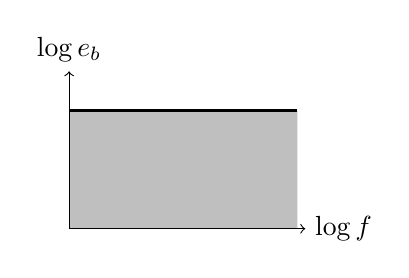
\begin{tikzpicture}
		\fill [gray!50, domain=0:2.9, variable=\x]
		(0, 0)
		-- plot ({\x}, {1.5})
		-- (2.9, 0)
		-- cycle;
		\draw[->] (0,0) -- (0,2) node[above]{$\log e_b$};
		\draw[->] (0,0) -- (3,0) node[right]{$\log f$};
		\draw[very thick] (0,1.5) -- (2.9,1.5);
		\end{tikzpicture}}
	\subfigure[Bruit rose]{\label{fig:bruitrose}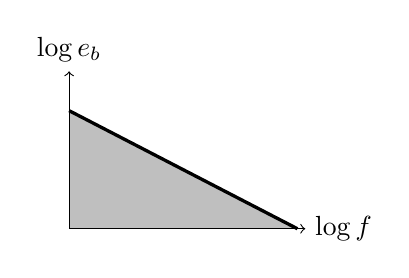
\begin{tikzpicture}
		\fill [gray!50, domain=0:2.9, variable=\x]
		(0, 0)
		-- plot ({\x}, {1.5-\x*0.51})
		-- (2.9, 0)
		-- cycle;
		\draw[->] (0,0) -- (0,2) node[above]{$\log e_b$};
		\draw[->] (0,0) -- (3,0) node[right]{$\log f$};
		\draw[very thick] (0,1.5) -- (2.9,0);
		\end{tikzpicture}}
	\caption{Répartition en fréquence de la densité spectrale de bruit}
\end{figure}
\subsubsection{Sommation de bruits divers}
Dans l'hypothèse où il n'y a pas corrélation entre:
\begin{itemize}
	\item les sources de bruits d'origine différente
	\item la même source à différentes fréquences
\end{itemize}
\centerline{$\Rightarrow$ Puissance totale de bruit = $\sum$ des puissance de bruit individuelles.}
Or la puissance de bruit $\propto$ valeur quadratique moyenne de la tension ou du courant de bruit $\rightarrow P_b=R \overline{I^2_b} = \frac{\overline{V_b^2}}{R}$. Il faut donc sommer \emph{quadratiquement} tensions et courants de bruit 
\[
V_b^2 = V_{b_1}^2 + V_{b_2}^2 + \dots + V_{b_n}^2 \qquad I_b^2 = I_{b_1}^2 + I_{b_2}^2 + \dots + I_{b_n}^2
\]
De même pour les densités spectrales:
\[
v_b^2(f) = v_{b_1}^2(f) + v_{b_2}^2(f) + \dots + v_{b_n}^2(f)
\]
\subsection{Types de bruit}
\subsubsection{Bruit thermique ou de Johnson}
Le bruit thermique est un bruit dû à l'agitation thermique des porteurs de charges ($e^-$ dans conducteur, $e^-+$ trous dans semi-conducteur). À $T>\SI{0}{\kelvin}$, il y a collision des porteurs de charges entre eux $\rightarrow$ répartition non uniforme des charges électriques $\rightarrow$ champ électrique variable aléatoirement.\\

Ses propriétés sont les suivantes:
\begin{itemize}
	\item {\makebox[6cm]{valeur moyenne nulle\hfill} $\overline{E_{bR}(t)}=0$} 
	\item {\makebox[6cm]{valeur quadratique moyenne\hfill} $\overline{E^2_{bR}(t)}=4kRT\Delta f$} avec $\left\{\substack{k\text{ : cst de Boltzmann }=\SI[per-mode=symbol]{1.374e-23}{\joule\per\kelvin}\\
	R \text{ : résistance en }\si{\ohm}\hfill \\
	T\text{ : température absolue en }\si{\kelvin}\hfill\\
	\Delta f\text{ : bande de fréquence observée}\hfill}\right.$
	\item bruit blanc
	\item existe dans toute résistance vraie
	\item mesurable malgré son faible ordre de grandeur\footnote{Potentiel du cerveau $\approx \SI{1}{\micro\volt}$}
\end{itemize}
\subsubsection{Bruits en 1/f}
Les bruits en 1/f sont plus fort à basses qu'à hautes fréquences (bruit rose), il en existe 2 types:
\begin{itemize}
	\item Bruit de scintillation:
	\begin{itemize}
		\item présent dans les semi-conducteurs
		\item d'origine incertaine, recombinaisons dans les défauts de surface du semi-conducteur ($e^-$ et trous)
	\end{itemize}
	\item Bruit en excès (ou bruit de constitution, "contact noise", "excess noise"):
	\begin{itemize}
		\item analogue au bruit de scintillation
		\item présent dans certaines résistances (ex. résistance à couche de carbones)
		\item engendré par l'évolution erratique (:= aléatoire) des lignes de courant (continu) dans un matériau non homogène
	\end{itemize}
\end{itemize}
\subsubsection{Autres types de bruit}
Le reste:
\begin{itemize}
	\item Bruit de grenaille (ou de Schottky):
	\begin{itemize}
		\item présent dans les semi-conducteurs
		\item dû à la nature quantifié du courant électrique, provoqué par passage des porteurs de charge au travers d'une barrière de potentiel
	\end{itemize}
	\item Bruit quantique:
	\begin{itemize}
		\item dû à la nature quantifiée de l'énergie rayonnée (photons)
	\end{itemize}
	\item Bruit de diffusion:
	\begin{itemize}
		\item présent dans les semi-conducteurs
		\item dû aux collisions des porteurs de charges avec le réseau cristallin
	\end{itemize}
	\item Bruit de génération/recombinaison:
	\begin{itemize}
		\item présent dans les semi-conducteurs
		\item  dû à la fluctuation aléatoire des taux de génération, des recombinaisons et des piégeages des porteurs
	\end{itemize}
	\item Bruit d'avalanche:
	\begin{itemize}
		\item présent dans les diodes Zener à tension d'avalanche élevée
		\item  dû au délogement de certains $e^-$ à cause d'$e^-$ accélérés par le champ électrique, venant créer des porteurs de charge supplémentaires (bruit important au voisinage de l'effet d'avalanche)
	\end{itemize}
	\item Bruit d'éclatement (ou bruit impulsif, "burst noise", "popcorn noise"):
	\begin{itemize}
		\item présent dans certains dispositifs électronique particulier (ex. diode tunnel)
		\item d'origine incertaine, liée aux défauts de fabrication
		\item Bruit non gaussien
	\end{itemize}
\end{itemize}
\subsection{Modélisation de bruit}
\paragraph{Dans un résistance:} la \autoref{fig:bruitresist} représente l'équivalent de Thévenin et de Norton pour le bruit thermique.
\begin{figure}[H] 
	\centering 
	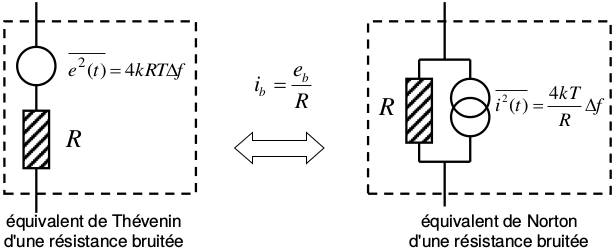
\includegraphics[width=0.8\textwidth,height=10\baselineskip,keepaspectratio]{ch3/image1} 
	\caption{Bruit thermique dans une résistance}
	\label{fig:bruitresist}
\end{figure}
\paragraph{Dans un transistor:} rappelons qu'un amplificateur différentiel est constitué de transistors. Les sources de bruits sont:
\begin{itemize}
	\item bruit thermique des résistances vraies ($R_{BB}'$)
	\item bruit de grenaille des courants (base et collecteur)
	\item bruit en 1/f du transistor
\end{itemize}
La modélisation du bruit est présenté à la \autoref{fig:bruittrans}.
\begin{figure}[H] 
	\centering 
	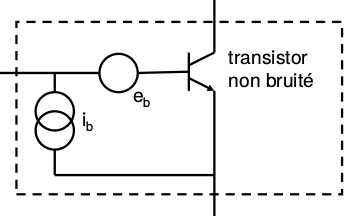
\includegraphics[width=0.8\textwidth,height=10\baselineskip,keepaspectratio]{ch3/image2} 
	\caption{Bruit dans un transistor}
	\label{fig:bruittrans}
\end{figure}
\paragraph{Dans un AOP:} rappelons qu'on AOP est constitué de résistances et de transistors. Le bruit est modélisé par la \autoref{fig:bruitaop}.
\begin{figure}[H] 
	\centering 
	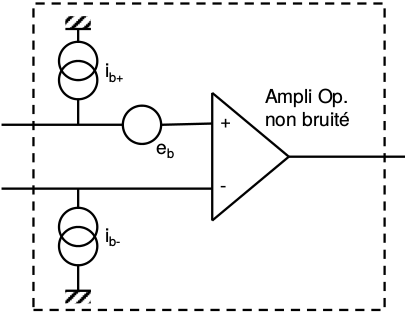
\includegraphics[width=0.8\textwidth,height=10\baselineskip,keepaspectratio]{ch3/image3} 
	\caption{Bruit dans un amplificateur opérationnel} 
	\label{fig:bruitaop}
\end{figure}
\paragraph{Remarques:} Les courants $i_{b^\pm} \neq$ courant de bias (= courant constant de polarisation). $i_{b^\pm}$ sont des courants à moyenne nulle, allant vers le circuit et dont l'impact dépend de l'impédance (+ l'impédance est grande, + le bruit est grand).
\subsection{Limitation de bruit}
\subsubsection{Introduction et principales techniques}
Le but de cette sous-section est de développer des méthodes afin de rendre l'amplitude du bruit négligeable face à celle du signal, c-à-d $\nearrow$ SNR. Pour ce faire, il est possible d'agir sur 2 choses:
\begin{enumerate}
	\item Augmenter le signal, c-à-d amplifier des que possible et autant que possible le signa $\Rightarrow$ pré-ampli à grand gain et faible bruit.
	\item Réduire le bruit de tous les composants.
\end{enumerate}
Afin de parvenir à un résultat, il est important de suivre ces quelques règles de bases:
\begin{enumerate}
	\item Cibler le type de bruit (afin de choisir des contre-mesures efficaces).
	\item S'attaquer au bruit prépondérant (on va peut-être s'occuper du gros d'abord, non ?).
	\item S'attaquer au bruit dès que possible (chaque module apportant son propre bruit (irréversible), il devient impossible de séparer les bruits entre eux au fur et à mesure que l'on avance sur la chaîne)
\end{enumerate}
Nous pouvons agir:
\begin{description}
\item \emph{au niveau des composants:}
\begin{itemize}
	\item Choisir des composants à faible bruit.
	\item Jouer sur les paramètres influençant directement le bruit (ex. réduire la température pour un bruit thermique).
\end{itemize}
\item \emph{au niveau du système:}
\begin{itemize}
	\item \hyperref[subsubsec:entreenobruit]{Pré-ampli à faible bruit} (parfois étage a transistor discrets afin de minimiser le bruit de l'aop, lui-même constitué d'un nombre conséquent de transistors discrets).
	\item \nameref{subsubsec:bandepass} (réduire le bruit dans un bande passante plus restreinte).
	\item \nameref{subsubsec:résistsource}.
	\item \nameref{subsubsec:detectsync} pour le bruit rose.
\end{itemize}
\end{description}
\subsubsection{Réduire la bande passante} \label{subsubsec:bandepass}

\subsubsection{Résistance de source} \label{subsubsec:résistsource}

\subsubsection{Étage d'entrée à faible bruit} \label{subsubsec:entreenobruit}

\subsubsection{Détection synchrone} \label{subsubsec:detectsync}

